\chapter{Experimental design}


\section{Introduction}

This chapter details the proposed methodological framework to produce medium-range predictions of areas at risk of flash floods over a continuous global domain. The framework follows a three-component approach, where each component builds upon the findings of the previous one, ensuring methodological coherence. This methodology also enables quantification of uncertainty at each stage of the methodological framework.

The first methodological component addresses the fundamental challenge that high-quality rainfall forecasts do not necessarily translate directly to accurate flash flood predictions. It therefore assesses the capability of medium-range global rainfall forecasts to identify areas at risk of flash floods up to medium-range lead times by proposing a flash-flood-focused rainfall verification framework. This initial verification is essential as it establishes the baseline predictive capacity of rainfall predictions from state-of-the-art global NWP models to identify areas at risk of flash flood risk.The second methodological component develops a machine learning model to identify areas at risk of flash floods over a continuous global domain. This data-driven approach represents a departure from traditional physically-based hydrological modelling, which often struggles with the computational demands and parameter uncertainty inherent in global-scale flash flood prediction. By utilising the Storm Event Database observations from the United States as training data, coupled with hydrological parameters from ERA5 reanalysis and precipitation characteristics from ERA5-ecPoint, the model establishes relationships between meteorological-hydrological conditions and observed flash flood occurrences. This approach capitalises on the relative abundance of flash flood observations in the United States whilst developing a framework that can be applied globally.
The third methodological component extends the application of the data-driven model to medium-range forecasts, enabling an assessment of flash flood predictability across extended forecast horizons. This component synthesises the findings from the previous two methods, applying the machine learning model framework to longer-range forecast data to evaluate how predictive skill for flash flooding decays with increasing lead time. This evaluation is crucial for understanding the temporal limitations of actionable flash flood predictions.

The following sections will detail each methodological component, including data sources, processing techniques, model development procedures, and verification frameworks. Particular attention is given to the challenges of developing a globally applicable model from geographically limited training data, and to the methodological considerations required for meaningful extension to medium-range forecasts and spatial coverage over a continuous global domain.






The primary objective of the experimental design chapter is to delineate the overarching experimental framework underpinning the research presented in this thesis. It articulates the sequential experimental strategy designed to address the interconnected research questions, weaving together the methodological and evaluation threads to present a cohesive and compelling research strategy. Hence, this chapter details the rationale, structure, and integrative approach to the experimental methods adopted, providing clarity on methodological decisions and interdependencies between various research stages (Figure \ref{fig:workflow_dataflow}), while detailed methodologies applied to answer each specific research question are described in the corresponding analytical chapters. This thesis adopts a thesis-by-publication format, with each core component of the research being prepared as a standalone peer-reviewed article, with the experimental framework prioritising the integration of findings from each phase, ensuring that the insights gained are effectively synthesised into a cohesive flash flood forecasting methodology. Hence, this chapter serves as a critical connector, integrating these individual publications into a coherent narrative that addresses the overarching thesis objective and ensures that the independent articles are effectively synthesised into a unified body of work. 

%%%%%%%%%%%%%%%%%%%%%%%%%%%%%%%%%%%%%%%%%%%%%%%%%%%%%%%%
\section{Integrated experimental workflow and data flow}

The methodological approach employed in this thesis is characterised by a deliberate integration of physical understanding and data-driven algorithms due to the recognition that, while traditional, physically-based models have laid the groundwork for flash flood prediction, they often struggle to capture the full complexity and variability of these events across diverse geographical and temporal scales. Machine learning, particularly deep learning, offers a powerful complementary tool for uncovering intricate patterns and relationships that conventional methods may overlook. However, data-driven methods are not pursued in isolation from physical understanding. Instead, the research methodology is grounded in a firm grasp of the underlying hydro-meteorological processes that contribute to flash flood occurrence, informing the selection of appropriate input variables, the design of the data-driven architectures, and the interpretation of the model outputs. This fusion of domain expertise and data-driven insights lies at the heart of the methodological framework, reflecting a commitment to developing a globally applicable, yet physically grounded flash flood forecasting system. Moreover, by embracing a mixed-methods approach, this research aims to generate a nuanced understanding of flash flood prediction that transcends the limitations of the single approaches. This methodological diversity is essential for achieving the overarching objective of developing a comprehensive, globally applicable flash flood forecasting system that can inform effective risk reduction strategies. 

The first phase, which addresses RQ1 in Chapter 5, defines a flash-flood-focused verification framework to assess the performance of global NWP rainfall forecasts in identifying areas at risk of flash floods up to medium-range lead times (up to day 10). This stage provides the flash-flood-focused verification framework that will be used throughout the thesis, and the benchmark performance against the (short-range) data-driven flash flood forecasts will be compared to. This is done in the recognition that a robust understanding of rainfall forecast performance in the identification of its capabilities in identifying areas at risk of flash flood is essential before pursuing more advanced prediction methods. By grounding the experimental framework in thorough rainfall forecast verification, the research establishes a solid foundation for subsequent developments. The objective verification framework uses flash flood impact observations as ground truth, so novel metrics are developed to handle the differences between continuous forecasts and binary observations, while accounting for the unique challenges posed by the rare and localised nature of flash floods. This analysis quantifies explicitly the uncertainties associated with existing prediction systems, providing a transparent assessment of their reliability and skill, informing the subsequent development of data-driven methods, in particular highlighting areas where data-driven techniques can offer significant improvements. A case-study-based approach is also used to provide in-depth insights into forecast performance differences between large-scale and small-scale (localised) flash flood events. The study was conducted at a regional level over continental Ecuador. To ensure the transferability of the findings from the Ecuador's example, the verification framework is designed to be modular and adaptable. The assessment metrics and criteria are selected based on their applicability to different geographical contexts, and the verification architecture is built to accommodate a wide range of data sources and formats. 

\begin{figure}[htbp]
\centering
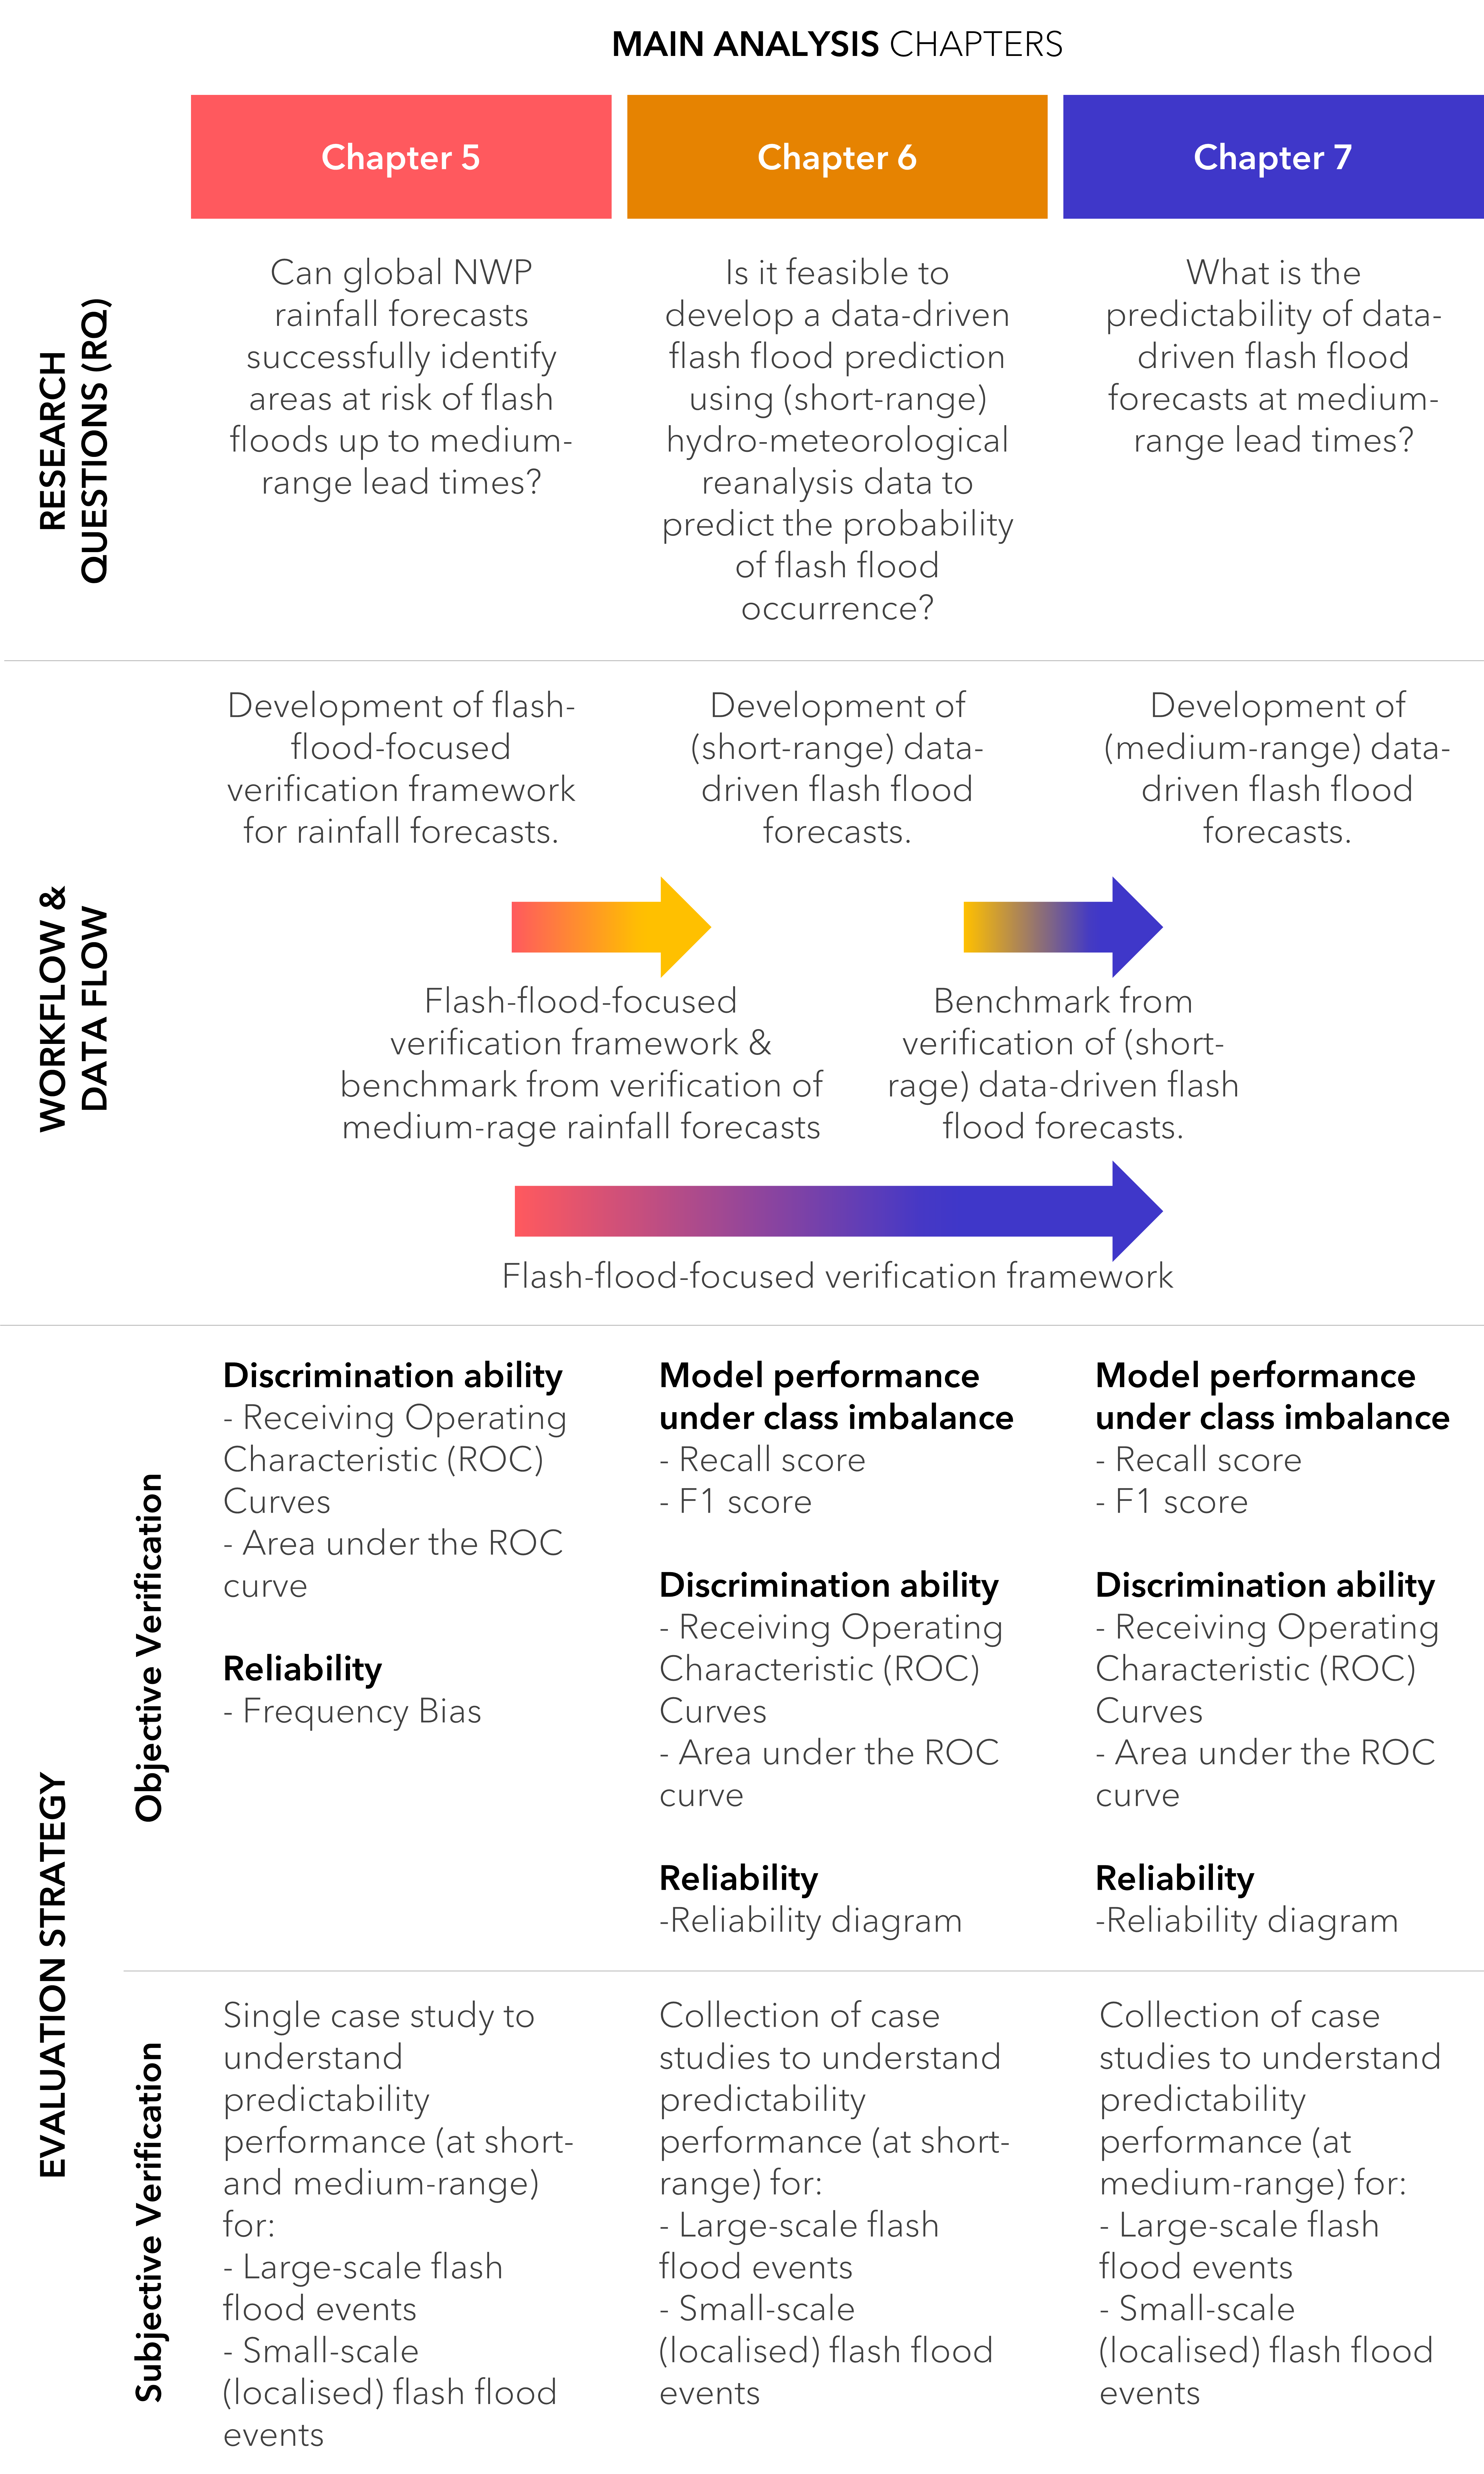
\includegraphics[scale=0.95]{Figures/Chapter_04/workflow_dataflow.png}
\caption{\textbf{Overview of the experimental design across the "Main Analysis" chapters (5 to 7).} The infographic delineates the research questions addressed in each chapter, the workflow of data flow across the chapters, and the adopted evaluation strategies to assess the performance of global NWP rainfall forecasts and data-driven flash flood predictions in identifying areas at risk of flash floods.}
\label{fig:workflow_dataflow}
\end{figure}

To assess the feasibility of developing (short-range) data-driven flash flood forecasts, which addresses RQ2 in Chapter 6, a machine learning model is developed using short-range hydro-meteorological reanalysis data and flash flood impact reports from NOAA's Storm Event Database. Different machine learning algorithms that handle complex non-linear relationships, such as decision trees and neural networks, were used. This phase leverages the wealth of hydro-meteorological data available through global reanalysis products, employing data-driven approaches to uncover complex patterns and relationships that contribute to flash flood development, and understand key drivers of flash flood occurrence across various geographical and climatological contexts. This study aims to create a robust and interpretable data-driven approach for analysing historical flash flood events by combining data-driven learning with physical understanding. 

Moreover, the concept here adopted relies on the fact that, for flash flood prediction, there is no need for complex machine learning algorithms that take account of spatio-temporal dependencies between different hydro-meteorological variables as it would be needed when modelling riverine floods, such as recurrent neural networks and long-short term memory neural networks, due to rapid reaction of flashy catchments to the triggering rainfall events. Hence, algorithms such as decision-tree-based models and feed-forward neural networks should be able to capture the hydro-meteorological processes that generate flash flood occurrence. Specific methods to account for data sparsity and imbalanced training datasets, such as oversampling (SMOTE) and undersampling (TOMEK), were considered and compared to the case of training over the imbalanced dataset. Moreover, due to the imbalanced training dataset, stratified k-fold cross-validation and hyper-parameter tuning were carried out to account for high uncertainty in estimating the model hyperparameters. The evaluation framework assesses the single machine learning algorithms separately and as an ensemble blend to understand whether ensemble stacking increases the single models' predictive skill. The same evaluation framework used in Chapter 5 was used to evaluate the (short-range) data-driven flash flood forecasts. For the objective verification, the flash flood impact reports from NOAA's Storm Event Database were used to compute verification scores to estimate the reliability and discrimination ability of the forecasts. Furthermore, specific scores, like recall and F1, were used to estimate the model's performance under class imbalance. Finally, subjective verification was carried out by defining a catalogue of case studies to assess the short-range predictability performance of the data-driven forecasts for large-scale and small-scale (localised) flash flood events. The verification results of the data-driven flash flood forecasts were benchmarked against the performance of single rainfall forecasts to identify areas at risk of flash floods. The study was conducted at a regional level in the contiguous US.  

To assess the predictability of the data-driven flash flood forecasts, which addresses RQ3 in Chapter 7, the machine learning model developed in Chapter 6 is applied over medium-range hydro-meteorological forecasts. Uncertainty and error growth for increasing lead times is evaluated and benchmarked against the (short-rage) data-driven flash flood forecasts. The same evaluation framework used in Chapter 5 and Chapter 6 was used to evaluate the medium-range data-driven flash flood forecasts.


%%%%%%%%%%%%%%%%%%%%%%%%%%%%%%%%%%%%%%%%%%%%%%%%%%%%
\section{Methodological assumptions and limitations} 

While the proposed flash flood forecasting system holds great promise for enhancing global prediction capabilities, it is essential to acknowledge and address methodological limitations inherent in the research design. This research acknowledges that flash floods are objective phenomena governed by physical laws but our understanding of them is shaped by the tools, methods, and data we have available. Acknowledging and managing these limitations is essential for ensuring the transparency, credibility, and usefulness of the research outcomes and guiding future improvements in the field of flash flood forecasting.

One of the primary limitations affecting all three studies is the availability and quality of hydro-meteorological data. Such limitation limits the accuracy and reliability of flash flood forecasts, which heavily depend on the spatial and temporal resolution, coverage, and consistency of the input data, such as rainfall observations, flash flood impact data, soil moisture measurements, and topographic information. In many regions, particularly developing countries, the scarcity of ground-based monitoring networks can introduce significant uncertainties in the modelling process. To address this limitation, the research will leverage multiple data sources, including post-processed rainfall global reanalysis that captures better localised rainfall extremes (ecPoint), and regional flash flood impact databases to reduce spatio-temporal uncertainties and uncovered regions.

The limited availability of hydro-meteorological data introduces high uncertainty in verifying flash-flood-focused global NWP rainfall forecasts and (short— and medium-range) data-driven flash flood predictions. The lack of comprehensive flash flood inventories, representing more closely the true frequency of flash flood events to define more consistent flash flood thresholds across different geographical settings, amplified by the rare and localised nature of flash floods, can hinder the objective assessment of forecast performance because it makes it difficult to accumulate sufficient samples for robust statistical verification. To overcome these verification challenges, this research will employ high-density regional flash flood impact databases in Ecuador and the US, where reporting times and locations have higher certainty and contain records spanning many decades. While we know this is not strictly true, we will assume that there are no spatial reporting biases. We will also assume that the reporting locations and times are correct because the grid spacing we are working with (ERA5, 31 km) and temporal resolution ( 24-hourly accumulation) already provide a good buffer around locations and reporting times. While some reports fall near the boundaries of the grid-boxes and the beginning/end of the accumulation period, this corresponds only to less than 5\% of the overall dataset, so we will not cater for such uncertainties. 

The integration of multiple data sources, physical models, and AI algorithms in the flash flood forecasting system can lead to the propagation and amplification of uncertainties through the various components of the system. To address the issue of uncertainty propagation, this research will implement an uncertainty quantification framework that accounts for aleatoric (inherent) and epistemic (knowledge-based) uncertainties in the forecasting system. This framework will involve ensemble modelling techniques, with multiple model runs performed with perturbed inputs and parameters to capture the range of possible outcomes. These techniques will be employed in defining the data-driven model for creating (short-range) flash flood predictions. Later, it will be used to assess how these uncertainties influence the error growth with lead time in the medium-range forecasts.
